\chapter{Introduction}

Zika virus is a member of the Flaviridae family
and the flavivirus genus, it is related to other mosquito borne viruses such as Dengue Virus, Yellow-Fever (YFV) virus  and West Nile virus \citep{doi}.The Virus originates from the Zika forest of Uganda and the first case was first isolated in 1947 from a rhesus monkey in the forest. Then later in 1954 a human was diagonised with the virus in Nigeria,\citep{2015zika}. Since then the virus has spread to different parts o the world. 
\begin{figure}[h!]
\centering
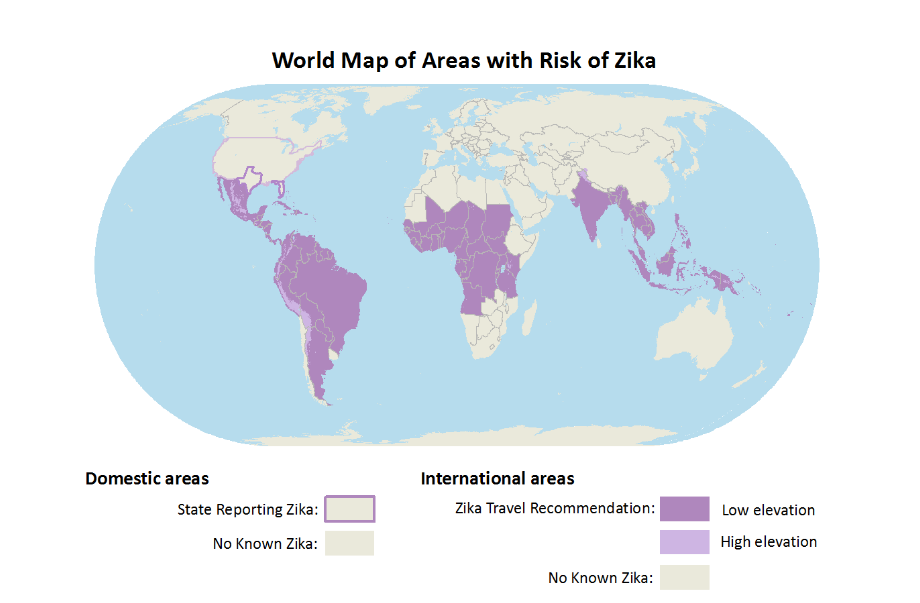
\includegraphics[scale=0.5]{images/map_zika.png} 
\caption{Counties with Zika Virus: Source CDC}\label{fig 1}
\end{figure}


Zika Virus is mainly spread by Aedes mosquitoes, when the Mosquito bites an infected person it carries the pathogen and when It bites an infected person it also it leaves the pathogen in them. Other ways of by which the virus spreads include, Blood transfusion, Unprotected Sex With an infected person and From mother to child, infected mothers can pass on the virus to their unborn children \citep{musso2014}.

\cite{musso2015}, shows that some of the symptoms are papular rash,fever,arthritis or arthralgia. In addition , headache, joint pain and red eyes are common symptoms of Zika virus. \cite{simoes2016zika} state adds that pregnant mothers who are infected with Zika during usually have child bearing defects. The Zika virus affect their foetus and development of the baby. Babies can face a range of neurologic sequelae suc as intellectual disability, hearing loss, vision loss, and seizures. These problems can range from mild to severe, are often life-long \citep{rasmussen2016zika}.

There is no known vaccination to prevent or treat for Zika virus. Prevention measures can be taken to prevent the spread of the virus. Preventing mosquito bites, this can be done by sleeping under a mosquito net, using mosquito replant, spraying mosquitos inside and outside among others. Another measure of prevention of Zika virus is practising safe sex and avoiding travelling to areas with high prevalence of Zika virus. Drugs for the systems of Zika are administered to patients as a way of treating Zika infected people because of the luck of a vaccination for the virus.


The spread of Zika virus has resulted in Zika epidemics in some part of the world as can be seen in figure \ref{fig 1} above. This cause a worry as the effects of an epidemic are more diver stating and if not controlled can affect the whole country region and World at large. 


 
 Mathematical models for disease transmission have been used to link biological processes of disease transmission and emergent of dynamics of infections at the population level. Researchers try to understand the environmental, biological  and behavioural infectiousness of a disease .
 
  Environmental infectiousness depends on geographical factors of an infected person. Some pathogens cannot survive inside or outside in given conditions. Thus some diseases or infections spread faster in certain weather conditions\citep{grass}. Understanding the timing and causes of seasonality offers important insights into how parasite–host systems interact how and when parasite control measures should be applied, and how disease risks will respond to anthropogenic climate change and altered patterns of seasonality \citep{altizer}. These factors must be captured in the models.
  
  Biological infectiousness depends on the pathogen's life cycle and the individual or host immune system. Some individuals have strong immune system against certain infections. This on the slows down the propagation the infection. On the other hand pathogens that live outside also affect the transmission dynamics of the infection.  The interaction of the genetic determinant of disease propagation in the pathogen and host is important in building model for the transmission dynamics of infectious diseases.
  
Behavioural infectiousness depends on the interaction behaviour of an individual. The contact pattern of the person affect how the individual is likely to propagate   the disease. Depending on the nature of disease transmission, if a persons has a lot of contact they are more likely to spread the disease to more people compared to one who has few contacts \citep{johnson2001sexual}. Contact in this context implies any interaction likely to result in the transmission of an infection.

The susceptibility of and individual largely depend on biological, environmental and behavioural factors of an individual. For example one's contact pattern, immunity and the environmental conditions will highly affect the probability of contracting an infection.

Epidemiologist together with mathematicians have for years been involved in infectious disease modelling to understand the dynamics of the spread of the disease and to come with measures of how the spread can be controls. Recently there has been a growing interest in modelling the spread of Zika virus \citep{ku2016}.

Over a  century, Mathematical representation and analysis of infectious diseases has been the centre of  infectious disease epidemiology \citep{b2005}. Differential equation have been used in the modelling of the dynamics of infectious diseases. They are base on the assumption of uniform mixing, that is everyone in the population has an equal probability of contracting an infectious disease \citep{kaplan2002emergency}.
Compartmental Mathematical models have been used to describe the transmission dynamic of Zika Virus \citep{gao2016}.

Mathematical modelling of infections diseases, started by the works of Daniel Bernoulli in \cite{bernoulli1760essai},in the quest to model the spread of small box and possible eradication. A century later the modelling become well established. The modelling of infectious disease dynamics is important for science and public policy among others. The models for infectious disease is helpful for prevention and planning the control of the spread of these disease. Policy makers use the information generated from the models in their policy formulation. In science it opens up new field of science and is vital in the study and development of drugs.

The dynamics of infectious disease propagation are modelled as dynamical system. A dynamical system is a system that evolves with time over a state space according to a fixed rule. Thus let $\mathbb{X}$ be a state space $\mathbb{T}$ set of times and $\mathbb{R}$ rule that specifies how the state evolves with time. the rule is a function that whose domain is $\mathbb{X} \mathbb{T}$ and co domain $\mathbb{X}$ that is,
\begin{equation*}
\mathbb{R}: \mathbb{X} \mathbb{T} \longrightarrow \mathbb{X}.
\end{equation*}

The population is characterized as $S(t)$, $E(t)$,$I(t)$ and $R(t)$ . Where $S(t)$ is the number of individuals susceptible but not infected at time $t$, $E(t)$ is the number of people exposed or infected but not infectious at time $t$, $I(t)$ is the number of infected and infectious people at time $t$ and $R(t)$ is the number of people removed from the ability of being infected.Removal is carried by either immunization,death,recovery from the disease. The epidemiological models can be classified as Susceptible,Infected and Recovered (SIR) , Susceptible Infected (SIS or SIS) , Susceptible -Exposed - Infectious and Removed (SEIR)  and any other intermediate category can be added.

The SIS model assumes that there is no immunity after recovery used to model infections where once a person recovers they become susceptible again for example infectious like flue. SIR model assumes that once a person recovers they become immune to the infection for example chicken pox. The SEIR assumes that onnce a person get becomes infected they do not  become infectious intermediately hence the intermediate compartment for exposed. 

The independent variable in the compartmental model is the time $t$ and the rates of transfer between compartments are expressed mathematically as a result models are formulated initially as differential equations. The most epidemic models are built on the SIR proposed by \cite{m1925applications}. The system can be written as;


\begin{center}
\begin{equation} \label{eqn1_1}
\left\lbrace \begin{array}{ccl}
\frac{dS}{dt} &= &-\alpha S_{(t)} I_{(t)},\\
 \frac{dI}{dt} &=& \alpha S_{(t)} I_{(t)} - \gamma  I_{(t)}, \\
 \frac{dR}{dt} &= &\gamma  I_{(t)},
\end{array} \right. 
\end{equation}
\end{center}

 with assumptions that there is homogeneous mixing in the population. That is the rate of new infections is proportional to the current numbers of susceptibles and infectives in the population. Which the main assumption deterministic models are built on. Deterministic population  models are models where the behaviour of the population of determined completely by history and the rules which govern the model. In formulating these models , in terms of derivatives of the sizes of the compartments and it is assumed that the number of members in each compartment is differentiable with time. This assumption is tenable only when the disease outbreak has been established  but not valid at the beginning of a disease out break when they are few infectives. When they are a few out breaks the number of infectious depends on random contacts of between small number of individuals.
 
 On the other hand Stochastic models are obtained by setting by adding a random variable called noise to the transmission dynamics of deterministic models.These random fluctuations may impact the evolution of the infection. Unlike deterministic model which assume homogeneous mix , an assumption which only holds in small populations. It is quiet unlikely that all people in will be equally susceptible to the disease and effective in spreading it \citep{ball1985deterministic}. A stochastic model can be further be described as a model in which the distribution of the length of the infectious period as allowed to have any distribution that can be describe by its Laplace transform \citep{addy1991generalized}.
 
 Lets an SIR compartmental model, for $t > 0$, $S(t),I(t),R(t)$ is the number of individuals in susceptible, infectious and removed. $N(t)$ the total number of particles at time $t$. The Poisson process, which is the underlying structure basic to the class of stochastic models and all Markov chain processes\citep{greenwood2009stochastic}. The individuals enter each compartment at random times and the initial fixed values , $S(0)$,$I(0)$ and $R(0)$ are fixed for some $\lambda > 0$. Letting $\beta$ to be the average number of  contacts an infectious person makes per unit of time that take leads to infection. The probability of a susceptible individual moving from compartment S to compartment I in the time interval $\left[ t,\triangle t \right]$ that is  S $\rightarrow S-1$ and I $\rightarrow I + 1 $ is $ \beta$ S I $ \triangle t + o (\triangle t)$. If it is assumed the an infected person recovers at the rate $\gamma$ hence the probability of an infected person moving from infected to recovered over an interval $\left[ t,\triangle t \right]$  given by $\gamma I_{t + \triangle t} -o (\triangle t)$ .It is known that,
 \begin{align*}
 N_t = S_t + I_t + R_t
 \\ \Rightarrow  R_t = N_t - S_t - I_t
\end{align*}  
Which implies that knowing $S_t,I_t$ is knowing $R_t$. Hence the model becomes an $S_t,I_t$ and thus the stochastic dynamical system can be written as;
 \begin{align}
 P((S_{t + \triangle t}, I_{t + \triangle t} - (S_t ,I_t) = ( - 1,1)) =  \beta S I  \triangle t + o (\triangle t).
 \\ P (((S_{t + \triangle t}, I_{t + \triangle t} - (S_t ,I_t) = ( 0,-1)) = \gamma I_{t + \triangle t} -o (\triangle t).
 \end{align}
 

Graph theory has over the years grown and has found its application many fields. A graph also known as a network   can be  defined as triple $G = (V,E,f)$ where $V$ is a finite set of nodes $E \subset V \oplus V = \left\lbrace e_1,e_2,\dots ,e_m \right\rbrace$ is a set and f is a mapping which associates some elements of $E$ to a pair of elements of $V$ \citep{estrada2012structure}. 

Some network properties that can be used to describe networks or graphs.A network is said to be connected if between any pair of node there exists a path. In modelling disease spread a connected network is one in which an infection could travel from one person to any other person in the network through some steps. Another property that is used to describe networks is distance. Distance between any two nodes in a network is defined as the length of the shortest path by each a node can be reached. This can be summed up as the average distance taken over al, pairs of individuals , which gives the idea of the typical distance between nodes in a network or the diameter of the graph which is the largest distance taken over all pairs \citep{chung2002average}.

The number of of neighbour is denoted by $k$ is known as the degree of connectivity. Looking at the entire population (space), the quantities  give a connectivity distribution. The degree is also describe as a mean and denoted by $<k>$.

Some other measures that can be used to describe a network measure are cliquishness, clustering coefficient, transitivity  coefficients and mutuality examine the extend to which the neighbourhood individual have a common neighbour,  leading to the appearance of triangles in  in the network.

 The concept of random graphs was first introduced by \cite{erdodblac1959ldquo}. A graph or network is said to have a small world property if it has a high clustering coefficient and a small average path length. This means that every node in the network can be connected with another using only few connections \citep{estrada2015first}. In 1967 there was an experiment carried out by Milgram, in which randomly selected individuals living in Kansas and Nabraska were asked to send a latter to someone in Boston, directly if they knew the person or through someone they new personally. It was found that the latter was sent through an average of 6 people and it was discovered that some acquaintances of an in individual were feeding the letter into back into the cycle \citep{travers1967small}.

A random graph can be defined as , given a $N$ number of vertices edges between them are drown such that between any pair $i,j$ there is an edge with uncorrelated probability $p$ \citep{newman2002random}. For example in \ref{fig:randomgraphs}, there are 3 random graphs with 10 vertices, with a probability of nodes $i,j$ being connect being 0, 0.5 and 0.8 in figure \ref{fig:a} \ref{fig:b} and \ref{fig:c} respectively. A random network model can exhibit the small world network property, it has an average degree $z= pN$. Random networks have a a low clustering coefficient $ c = \frac{z}{N}$ \citep{newman2003structure}.

Classical models are built on an assumption of full mixture , random networks on the other hand are said to be well mixed. Thus they have a much lower epidemic threshold than the expected real world population \citep{witten2007simulations}.
\begin{figure}[h]
    \centering
    \begin{subfigure}[b]{0.3\textwidth}
        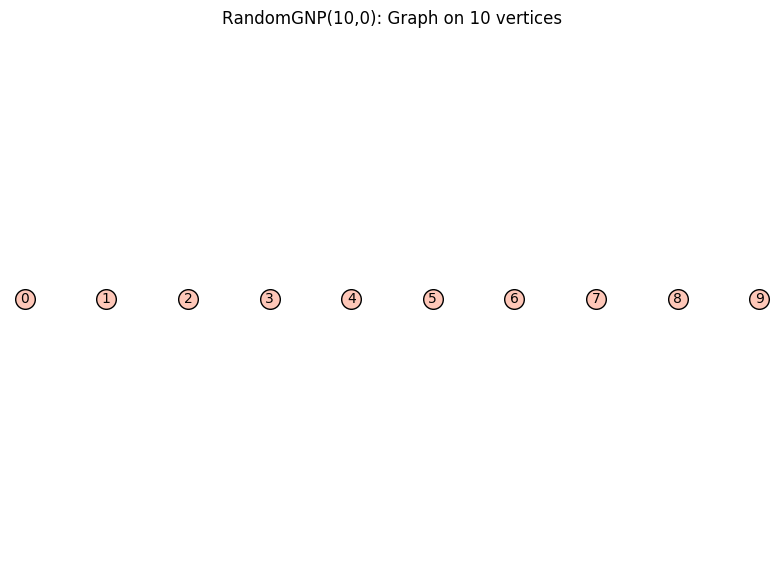
\includegraphics[scale=0.3]{images/rgraph2.png} 
        \caption{ $p =0$}
        \label{fig:a}
    \end{subfigure}
    ~ %add desired spacing between images, e. g. ~, \quad, \qquad, \hfill etc. 
      %(or a blank line to force the subfigure onto a new line)
    \begin{subfigure}[b]{0.3\textwidth}
        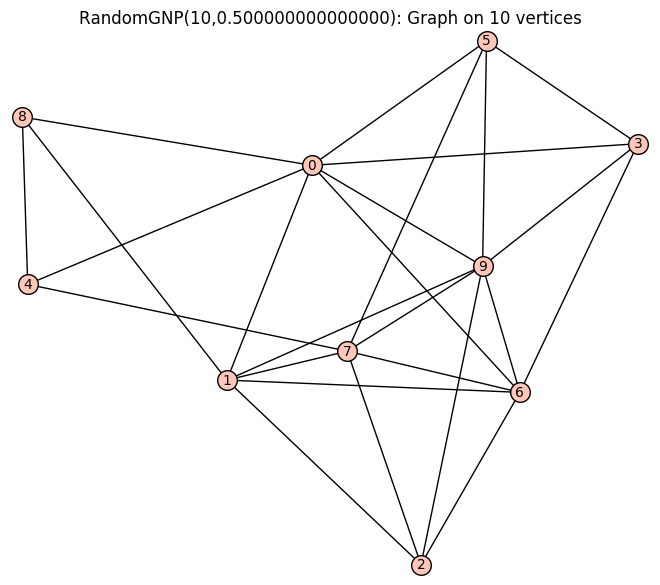
\includegraphics[width=\textwidth]{images/rgraph1.png}
        \caption{$p=0.5$}
        \label{fig:b}
    \end{subfigure}
    ~ %add desired spacing between images, e. g. ~, \quad, \qquad, \hfill etc. 
    %(or a blank line to force the subfigure onto a new line)
    \begin{subfigure}[b]{0.3\textwidth}
        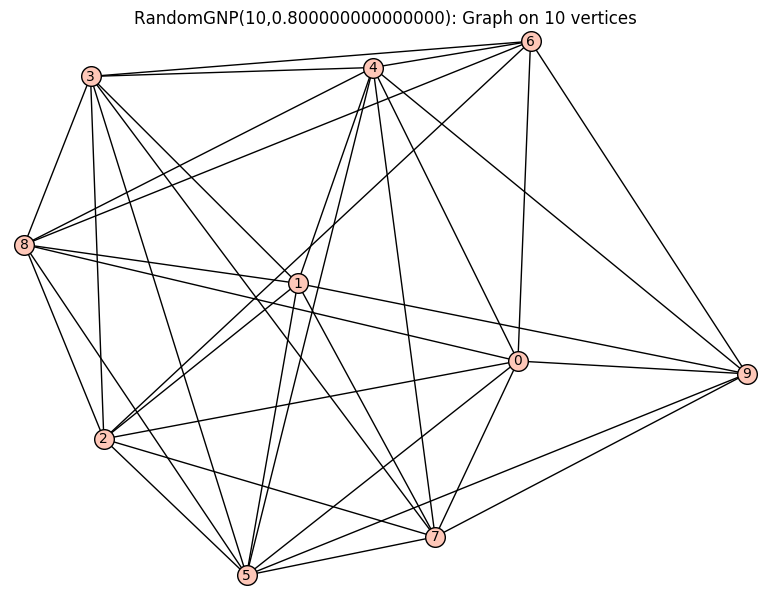
\includegraphics[width=\textwidth]{images/rgraph3}
        \caption{$p= 0.8$}
        \label{fig:c}
    \end{subfigure}
    \caption{Random Graphs}\label{fig:randomgraphs}
\end{figure}


In addition to Random graphs there are other networks on which epidemiology models have been built on   Watts–Strogatz, lattice,Barabasí–Albert, and power-law or “scale-free” \citep{witten2007simulations}. These networks have a small world properties except for the Barabasí–Albert network.The model have different network structures and network statistics, which is not the scope of this paper.


Regular lattices and random graphs have a long history of use in network theory and to model population structures,\cite{harris1974contact}  gives an example of classic lattice. Models built on latices assume that individuals are located as nodes on a regular lattice and connections are made of some collection of near neighbours or each node. For example people may be spread out such that connections are made to their four nearest neighbours, one on the left,right, up and down this is called a Neuman neighbours  or eight neighbours where four diagonal elements are added to the Neuman neighbours and this is called the Moore neighbour hood \citep{lloyd2006infection}.To avoid the effect of the nodes at the end not being connected the last and first neighbours are made neighbours.

The main difference between a random graph and lattices is that interactions are local, that is individuals are only related to their neighbours. Where as in random networks the connections are made are global, that is connections are made without taking spatial locations of an individual into consideration. 


Small world networks  were first introduced by Watts and Strogatz as an intermediate between the regular lattice and randomly rewiring certain proportions $p$ of the network links\citep{watts1998collective}. The small world networks allows for random contacts across the network. That is in addition to near neighbours as in a regular lattice, each node has a random distant neighbour connected to it \citep{watts1998collective}.

 
 on the other hand assume that one is more likely to spread the disease to someone in their family, someonewho lives near the, or someone you they. It combines this sort of clustering in the graph with a probability to model the spread of disease as a dynamical system \citep{newman2001random}.


In this research we will compare the traditional epidemiological model based on Random network assumption and the Small world networks to model the population Dynamics in the spread of Zika Virus. This infection of of Zika virus will be modelled using the SEIR compartmental model based on the two assumptions of transmission. Then real life data will be fit on both models to validate each model and to test which on is better.

